\anexo{Resultados de la encuesta}

Las figuras siguientes corresponden a los resultados de la encuesta desarrollada; el análisis completo se encuentra en el Capítulo 4, Sección~\ref{sec:encuesta-usuarios}.

\begin{figure}[htbp]
    \centering
    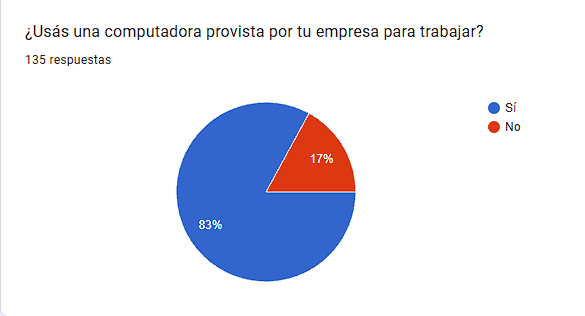
\includegraphics[width=0.8\textwidth]{images/Imagenes_encuestas/1.png}
    \caption{¿Usás una computadora provista por tu empresa para trabajar? (n=135)}
    \label{fig:encuesta-1}
\end{figure}

\begin{figure}[htbp]
    \centering
    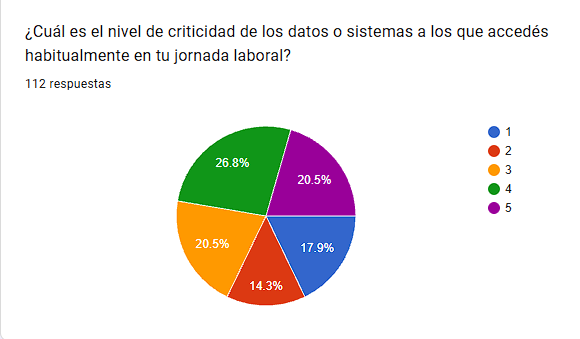
\includegraphics[width=0.8\textwidth]{images/Imagenes_encuestas/2.png}
    \caption{Nivel de criticidad de los datos o sistemas a los que accede habitualmente (n=112)}
    \label{fig:encuesta-2}
\end{figure}
\FloatBarrier

\begin{figure}[htbp]
    \centering
    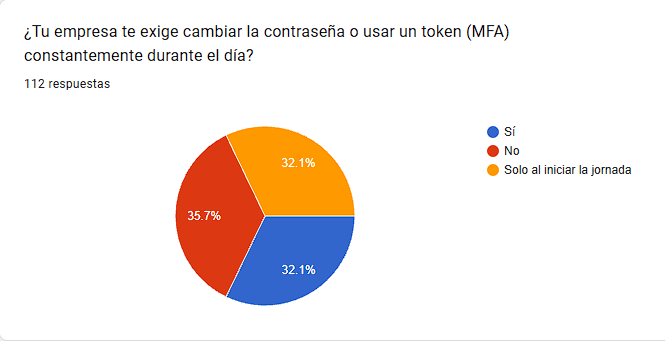
\includegraphics[width=0.8\textwidth]{images/Imagenes_encuestas/3.png}
    \caption{¿Tu empresa te exige cambiar la contraseña o usar un token (MFA) constantemente durante el día?}
    \label{fig:encuesta-3}
\end{figure}

\begin{figure}[htbp]
    \centering
    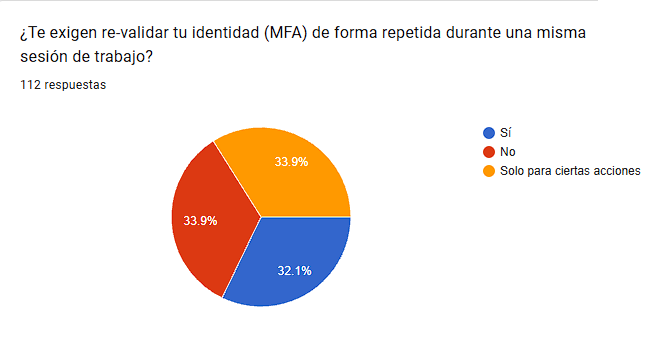
\includegraphics[width=0.8\textwidth]{images/Imagenes_encuestas/4.png}
    \caption{¿Te exigen re-validar tu identidad (MFA) de forma repetida durante una misma sesión?}
    \label{fig:encuesta-4}
\end{figure}

\begin{figure}[htbp]
    \centering
    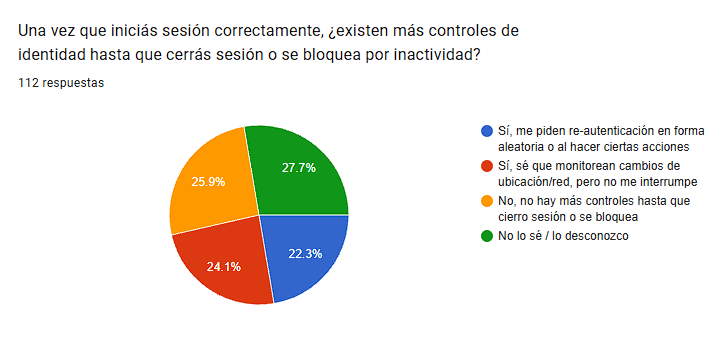
\includegraphics[width=0.8\textwidth]{images/Imagenes_encuestas/5.png}
    \caption{Una vez iniciada sesión correctamente, ¿existen más controles de identidad hasta el cierre o bloqueo por inactividad?}
    \label{fig:encuesta-5}
\end{figure}

\begin{figure}[htbp]
    \centering
    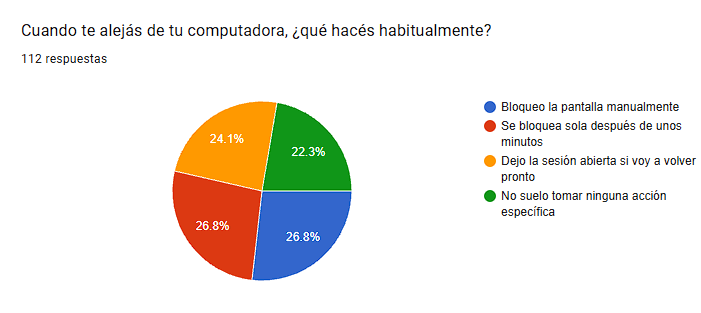
\includegraphics[width=0.8\textwidth]{images/Imagenes_encuestas/6.png}
    \caption{Cuando te alejás de tu computadora, ¿qué hacés habitualmente?}
    \label{fig:encuesta-6}
\end{figure}

\begin{figure}[htbp]
    \centering
    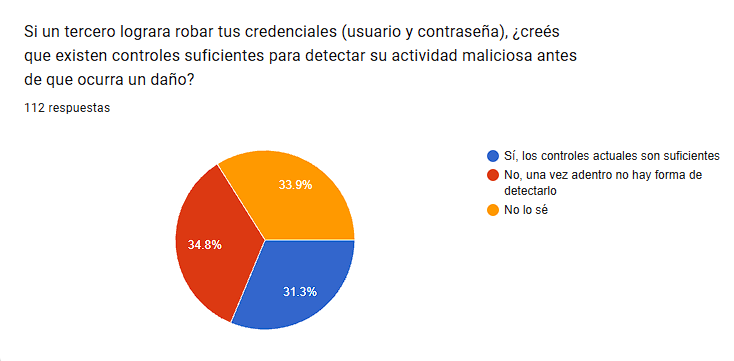
\includegraphics[width=0.8\textwidth]{images/Imagenes_encuestas/7.png}
    \caption{Si un tercero robara tus credenciales, ¿creés que existen controles suficientes para detectar su actividad maliciosa antes de que ocurra un daño?}
    \label{fig:encuesta-7}
\end{figure}
\FloatBarrier

\begin{figure}[htbp]
    \centering
    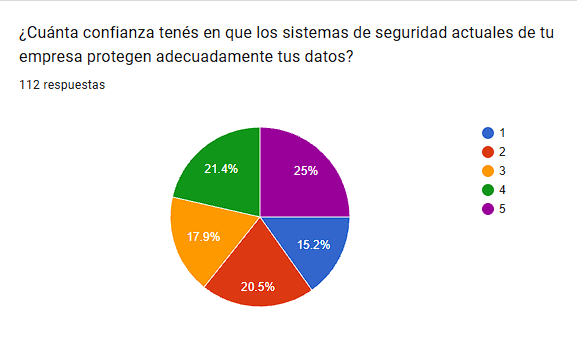
\includegraphics[width=0.8\textwidth]{images/Imagenes_encuestas/8.png}
    \caption{¿Cuánta confianza tenés en que los sistemas de seguridad actuales de tu empresa protegen adecuadamente tus datos?}
    \label{fig:encuesta-8}
\end{figure}

\begin{figure}[htbp]
    \centering
    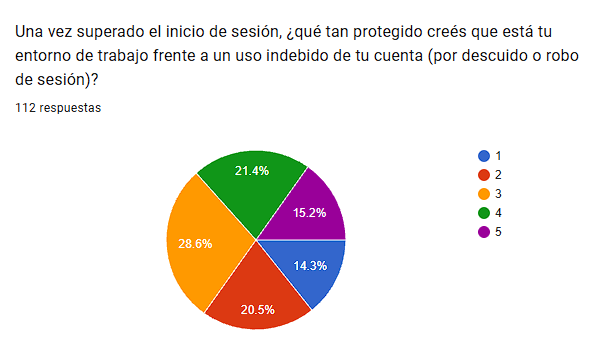
\includegraphics[width=0.8\textwidth]{images/Imagenes_encuestas/9.png}
    \caption{Una vez superado el inicio de sesión, ¿qué tan protegido creés que está tu entorno de trabajo frente a un uso indebido de tu cuenta?}
    \label{fig:encuesta-9}
\end{figure}
\FloatBarrier

\begin{figure}[htbp]
    \centering
    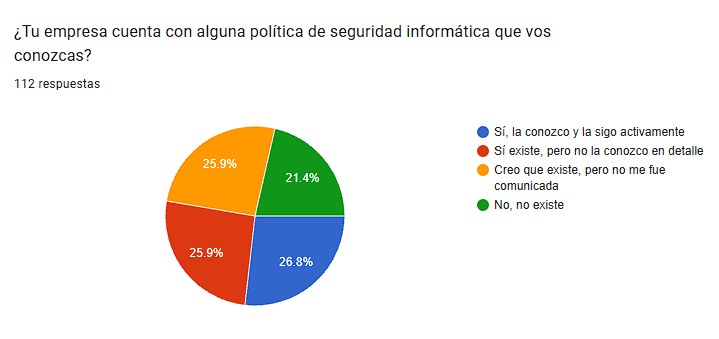
\includegraphics[width=0.8\textwidth]{images/Imagenes_encuestas/10.png}
    \caption{¿Tu empresa cuenta con alguna política de seguridad informática que vos conozcas?}
    \label{fig:encuesta-10}
\end{figure}

\begin{figure}[htbp]
    \centering
    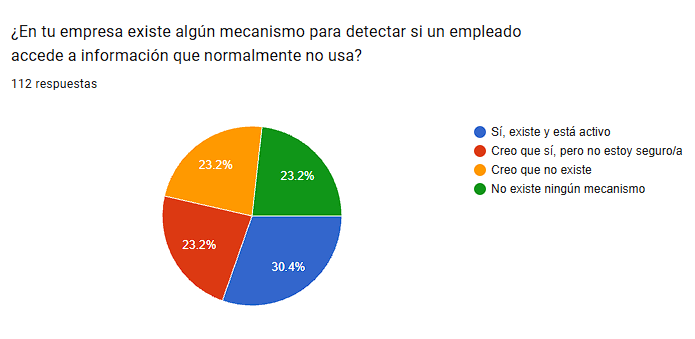
\includegraphics[width=0.8\textwidth]{images/Imagenes_encuestas/11.png}
    \caption{¿En tu empresa existe algún mecanismo para detectar si un empleado accede a información que normalmente no usa?}
    \label{fig:encuesta-11}
\end{figure}
\FloatBarrier

\begin{figure}[htbp]
    \centering
    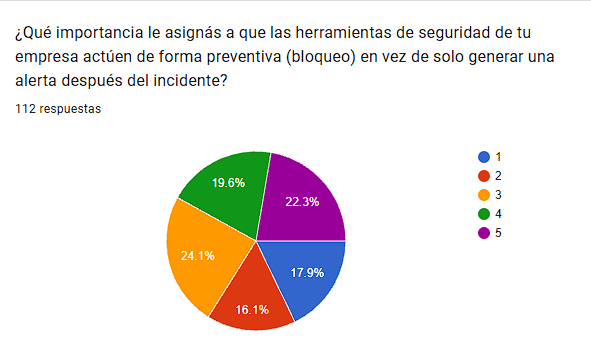
\includegraphics[width=0.8\textwidth]{images/Imagenes_encuestas/12.png}
    \caption{¿Qué importancia le asignás a que las herramientas de seguridad actúen de forma preventiva (bloqueo) en vez de solo alertar después del incidente?}
    \label{fig:encuesta-12}
\end{figure}

\begin{figure}[htbp]
    \centering
    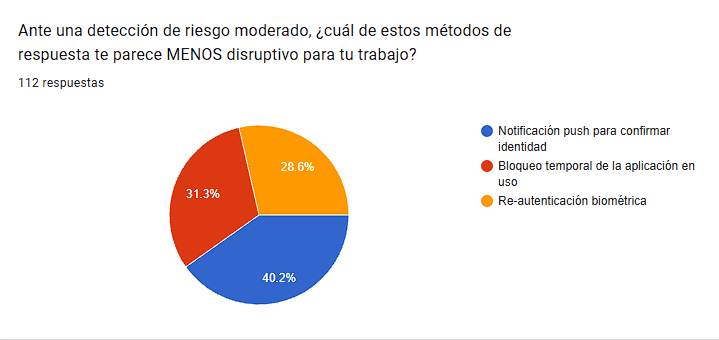
\includegraphics[width=0.8\textwidth]{images/Imagenes_encuestas/13.png}
    \caption{Ante una detección de riesgo moderado, ¿cuál de estos métodos de respuesta te parece MENOS disruptivo para tu trabajo?}
    \label{fig:encuesta-13}
\end{figure}
\FloatBarrier

\begin{figure}[htbp]
    \centering
    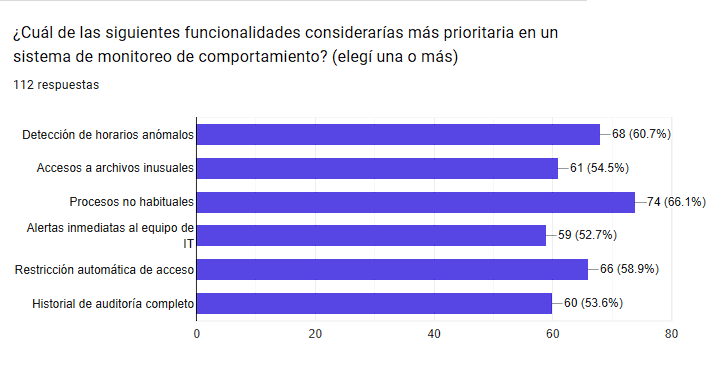
\includegraphics[width=0.8\textwidth]{images/Imagenes_encuestas/14.png}
    \caption{¿Cuál de las siguientes funcionalidades considerarías más prioritaria en un sistema de monitoreo de comportamiento? (elegí una o más)}
    \label{fig:encuesta-14}
\end{figure}
\FloatBarrier

\begin{figure}[htbp]
    \centering
    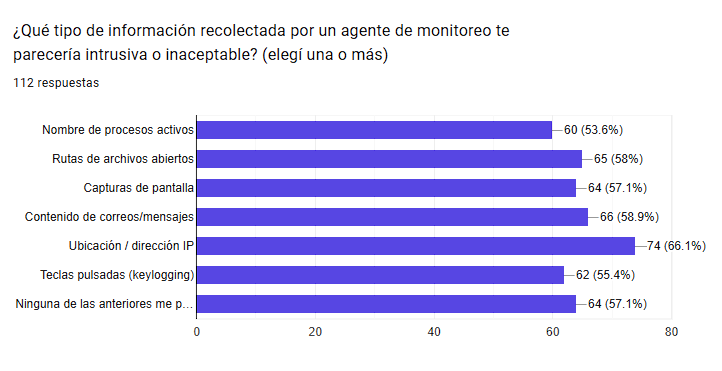
\includegraphics[width=0.8\textwidth]{images/Imagenes_encuestas/15.png}
    \caption{¿Qué tipo de información recolectada por un agente de monitoreo te parecería intrusiva o inaceptable? (elegí una o más)}
    \label{fig:encuesta-15}
\end{figure}

\begin{figure}[htbp]
    \centering
    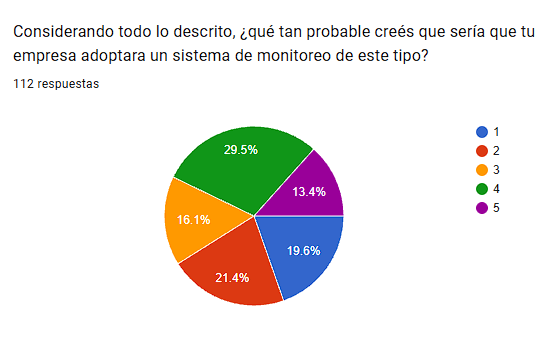
\includegraphics[width=0.8\textwidth]{images/Imagenes_encuestas/16.png}
    \caption{¿Qué factor sería más determinante para que tu empresa adopte o rechace un sistema de monitoreo conductual?}
    \label{fig:encuesta-16}
\end{figure}
\FloatBarrier

\begin{figure}[htbp]
    \centering
    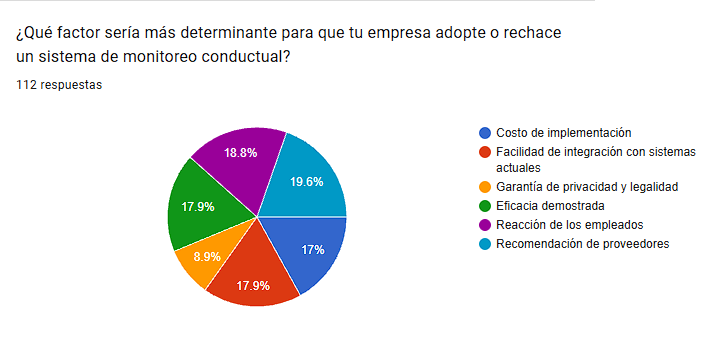
\includegraphics[width=0.8\textwidth]{images/Imagenes_encuestas/17.png}
    \caption{Considerando todo lo descrito, ¿qué tan probable creés que sería que tu empresa adoptara un sistema de monitoreo de este tipo?}
    \label{fig:encuesta-17}
\end{figure}
\FloatBarrier

\begin{figure}[htbp]
    \centering
    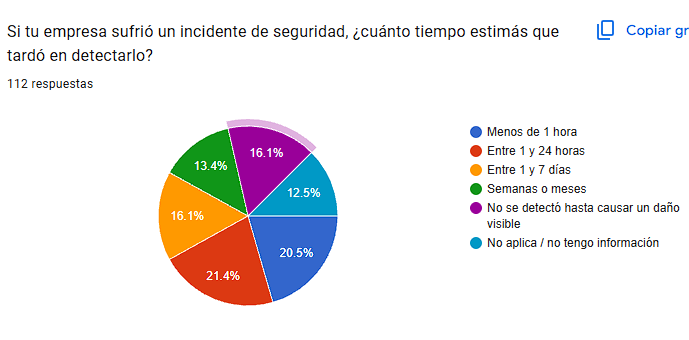
\includegraphics[width=0.8\textwidth]{images/Imagenes_encuestas/18.png}
    \caption{Si tu empresa sufrió un incidente de seguridad, ¿cuánto tiempo estimás que tardó en detectarlo?}
    \label{fig:encuesta-18}
\end{figure}
\FloatBarrier
